%% Manuscript for Physical Review E
%% Physical Boundaries of Biological Tryptophan Networks
%% Revised and expanded version

\documentclass[aps,pre,twocolumn,showpacs,superscriptaddress]{revtex4-2}
\usepackage[T1]{fontenc}
\usepackage{lmodern}
\usepackage{graphicx}
\usepackage{microtype}
\usepackage{xurl}
\usepackage{amsmath}
\usepackage{amssymb}
\usepackage{textcomp}
\usepackage[hidelinks]{hyperref}
\usepackage{booktabs}
\usepackage{placeins}


\begin{document}

\title{Physical Boundaries of Biological Tryptophan Networks: Non-Radiative Excitonic Energy Hopping vs.~Free-Space Optical Signaling}

\author{Dhiraj Kumar}
\author{Niraj Kumar}
\affiliation{Independent Researcher}

\date{\today}

\begin{abstract}
We analyze the physical limits of energy transfer in neural tryptophan (Trp) networks using 20 cryo-EM and X-ray structures from the Protein Data Bank. Energy transfer is characterized by two distinct regimes separated by a critical distance of $\sim1.5$~nm: (i) non-radiative dipole-dipole coupling (F\"orster resonance energy transfer, FRET) dominates at sub-$1.5$~nm separations, with efficiency $E_{\mathrm{FRET}} > 0.90$ for the closest Trp pairs; (ii) free-space radiative transfer is highly inefficient beyond $2$~nm, with probability $P_{\mathrm{free}} < 10^{-5}$ per exciton due to $1/r^2$ geometric spreading, ultraviolet tissue attenuation ($\alpha \sim 1000$~m$^{-1}$), and spectral mismatch between Trp emission ($\sim320$--$350$~nm) and candidate acceptor absorption bands. Pair-distance histograms from four representative PDB targets show that adjacent Trp residues cluster at $0.6$--$1.3$~nm, placing them in the FRET-dominated regime. Using PDB coordinates to compute dipole coupling matrices, we find coupling strengths of $J_{ij} \approx 150$--$300$~cm$^{-1}$ for the closest pairs, corresponding to exciton hopping times of $18$--$35$~fs. This work establishes a two-regime analysis: free-space optical Trp-Trp coupling is highly inefficient, while non-radiative FRET at sub-$1.5$~nm distances within low-dielectric hydrophobic pockets ($\varepsilon \approx 2$) is structurally viable and quantified from PDB data.
\end{abstract}

\maketitle

\section{Introduction}
\label{sec:intro}

A recurring hypothesis in the biophotonics literature proposes that ultra-weak photon emissions (UPE) from cellular metabolism serve a functional signaling role. Popp and colleagues~\cite{Popp1992} first suggested that biophotons could mediate intercellular communication. Tang and Dai~\cite{Tang2014} demonstrated that biophotons propagate along nerve roots and proposed a light-based communication system operating alongside electrical signaling. More recently, Babcock and Kurian~\cite{Babcock2024} showed that dense tryptophan (Trp) networks in microtubules support room-temperature superradiance, and Patwa et al.~\cite{Patwa2024} demonstrated quantum-enhanced photoprotection in neuroprotein architectures. These studies suggested that Trp emissions could serve biological signaling functions by routing optical information through aromatic networks.

We quantitatively evaluate that hypothesis. Using measured absorption cross-sections, waveguide optics, and the Stokes shift between Trp absorption (280~nm) and emission (327~nm), we compute an upper bound on free-space radiative Trp-to-Trp energy transfer. The result shows that free-space optical coupling between Trp cores is highly inefficient under cellular conditions. We then characterize the alternative non-radiative regime (FRET) that dominates at sub-$1.5$~nm separations, quantified directly from PDB structural data.

\section{Results}

\subsection{Structural Trp Networks in Neural Receptors}

We analysed 20 cryo-EM and X-ray structures from the Protein Data Bank (PDB), spanning ligand-gated and voltage-gated ion channels, GPCRs, synaptic vesicle anchors, cytoskeletal filaments, and membrane transporters. For each structure, we extracted the coordinates of all Trp residues (using the CG atom of each indole ring as a geometric proxy, with an estimated $\pm 0.3$~nm boundary uncertainty due to side-chain rotamers) and computed the full pair-distance matrix. Pairs with centre-to-centre separation $< 1.5$~nm were classified as quantum-coupled (permitting exciton hopping via dipole-dipole interaction); pairs with $1.5$--$5$~nm separation were classified as optical relay candidates (accessible via biophoton signaling).

Table~\ref{tab:structural} summarises the Trp network topology of each target.

\begin{table*}[htbp]
\caption{Structural properties of Trp networks in 19 proteins. ``Coupled pairs'' have $R < 1.5$~nm; ``relay pairs'' have $1.5 \leq R \leq 5$~nm. Four targets with $<2$ Trp lacked sufficient density for pair analysis. Human brain proteins are marked with $\dagger$. Pair counts near the $1.5$~nm cutoff have an estimated $\pm 0.3$~nm boundary uncertainty due to side-chain rotamers. The uncertainties on coupled and relay pairs are anti-correlated: a pair crossing the $1.5$~nm boundary changes the coupled count by $\pm1$ and the relay count by $\mp1$, conserving the total $\binom{N}{2}$ pair sum.}
\label{tab:structural}
\centering
\begin{tabular}{llcccc}
\toprule
PDB & Protein & Source & Trp & Coupled & Relay \\
\midrule
6HUO & GABA$_A$ receptor $\alpha1\beta3\gamma2$ & Human brain$\dagger$ & 26 & $11\pm4$ & $314\pm4$ \\
6IRA & NMDA receptor GluN1/GluN2A & Human brain$\dagger$ & 28 & $16\pm5$ & $362\pm5$ \\
6AGF & Na$_V$1.4 sodium channel & Human (skeletal muscle) & 28 & $20\pm6$ & $358\pm6$ \\
2BG9 & nACh receptor & \emph{T. marmorata} (electric ray) & 31 & $19\pm7$ & $446\pm7$ \\
7KOX & $\alpha$7 nicotinic AChR & Human brain$\dagger$ & 12 & $4\pm2$ & $62\pm2$ \\
3KG2 & AMPA receptor GluA2 & Rat (neural) & 12 & $3\pm2$ & $63\pm2$ \\
2A79 & K$_V$1.2 potassium channel & Rat (neural) & 11 & $10\pm3$ & $45\pm3$ \\
5C1M & $\mu$-opioid receptor & Human brain$\dagger$ & 9 & $3\pm2$ & $33\pm2$ \\
6PM6 & Glycine receptor $\alpha1$ & Zebrafish & 7 & $3\pm2$ & $18\pm2$ \\
5SVK & P2X$_3$ purinergic receptor & Human (sensory) & 4 & $1\pm1$ & $5\pm1$ \\
\addlinespace
5GJV & Ca$_V$1.1 calcium channel & Rabbit (skeletal muscle) & 42 & $23\pm11$ & $838\pm11$ \\
4PE5 & NMDA receptor GluN1/GluN2B & Rat (neural) & 18 & $10\pm4$ & $143\pm4$ \\
1U19 & Rhodopsin & Bovine (retinal) & 5 & $2\pm1$ & $8\pm1$ \\
1BL8 & KcsA K$^+$ channel & Bacterial & 5 & $3\pm1$ & $7\pm1$ \\
3GD8 & Aquaporin-4 & Human brain (glial)$\dagger$ & 5 & $3\pm1$ & $7\pm1$ \\
1JFF & Tubulin $\alpha\beta$ dimer & Porcine (ubiquitous) & 5 & $1\pm1$ & $9\pm1$ \\
3N2K & Tubulin $\alpha\beta$ dimer & Mammalian (ubiquitous) & 5 & $1\pm1$ & $9\pm1$ \\
3J5P & TRPV1 ion channel & Rat (sensory) & 5 & $1\pm1$ & $9\pm1$ \\
1SFC & SNARE complex & Rat (neural) & 2 & $1\pm1$ & $0\pm0$ \\
\bottomrule
\end{tabular}
\end{table*}

Of the 19 targets surveyed, 17 contain 4--42 Trp residues, with the number of quantum-coupled pairs per structure ranging from 1 to 23. Dense Trp networks are common across diverse protein families, but the relationship with signaling speed is more complex than a simple correlation: the fastest synapses (nAChR, Na$_V$1.4, NMDA) have high Trp counts (28--31), yet the slow Ca$_V$1.1 calcium channel has the highest Trp count in the dataset (42 Trp, 23 coupled pairs). Small signaling complexes such as SNARE (2 Trp, 1 coupled) and P2X$_3$ (4 Trp, 1 coupled) have minimal Trp networks. The pair counts in Table~\ref{tab:structural} should be interpreted with a boundary uncertainty of approximately $\pm 0.3$~nm near the $1.5$~nm cutoff due to the CG atom proxy for the indole ring center (see Methods). For typical targets, this translates to an uncertainty of $\pm 1$--$11$ pairs in the coupled column, with the largest absolute uncertainties for targets with the most Trp residues.

\subsection{Proof of Free-Space Infeasibility}

\subsubsection{Upper bound on Trp-to-Trp radiative transfer}

We first evaluate the possibility of long-range radiative signaling between Trp sites at intercellular or inter-protein separations ($r > \lambda/2\pi \approx 52$~nm for 327~nm light). At these distances, far-field absorption cross-sections and geometric optics are valid. The subsequent section addresses the sub-$1.5$~nm regime where near-field dipole-dipole coupling dominates.

A Trp exciton at the absorption peak (280~nm, $35\,700$~cm$^{-1}$) undergoes radiative relaxation with Stokes shift to the emission peak (327~nm). The measured quantum yield for Trp in polymerized tubulin is $QY = 0.21$~\cite{Babcock2024}. The expected number of emitted photons per absorbed photon is therefore $n_{\mathrm{gen}} = QY \approx 0.21$. We caution that this $QY$ is measured in tubulin and may differ for membrane-bound ion channels due to local quenching environments.

Only a fraction of these photons are captured by the lipid membrane waveguide due to total internal reflection constraints. The capture fraction is determined by the critical angle $\theta_c = \arcsin(n_{\mathrm{cytoplasm}} / n_{\mathrm{lipid}})$ for the interface between the lipid core ($n_{\mathrm{lipid}} \approx 1.45$) and the aqueous cytoplasm ($n_{\mathrm{cytoplasm}} \approx 1.33$):

\[
f_{\mathrm{capture}} = \cos\theta_c \approx 0.40.
\]

The Trp absorption cross-section at the emission wavelength is obtained from the measured extinction coefficient at 280~nm ($\varepsilon \approx 5600$~M$^{-1}$cm$^{-1}$) scaled by the Gaussian absorption lineshape:

\[
\sigma_{327} = \sigma_{280} \,
\exp\!\left[-\frac{1}{2}\left(\frac{47}{21.2}\right)^2\right] 
\approx 1.8\times10^{-22}~\mathrm{m}^2,
\]

where $\sigma_{\mathrm{FWHM}} = 21.2$~nm is the Gaussian standard deviation (FWHM $\approx 50$~nm for Trp). Combining these, the per-exciton Trp-to-Trp re-excitation probability is:
\begin{equation}
p_{\mathrm{trp}} = n_{\mathrm{arr}} (\sigma_{327}/A_{\mathrm{target}}) \approx 1.5\times10^{-5},
\label{eq:ptrp}
\end{equation}

where $A_{\mathrm{target}} \approx 1$~nm$^2$ is the effective target area and $n_{\mathrm{arr}} = n_{\mathrm{gen}} \times f_{\mathrm{capture}}$ is the expected number of photons arriving at the target. Since $n_{\mathrm{arr}} \ll 1$, the linear approximation is exact to first order, and the binomial form $(1-p)^n$ reduces to $n \cdot p$. This bound assumes adjacent Trp sites (no geometric spreading factor); for sites separated by distance $r$, the probability decreases as $1/r^2$ as given in the two-regime function below.

The low probability ($p \approx 1.5\times10^{-5}$) is the central result: free-space radiative Trp-to-Trp energy transfer faces severe physical limitations under cellular conditions. This upper bound depends primarily on measured quantities (absorption cross-section $\sigma_{280} = 2.1\times10^{-21}$~m$^2$, quantum yield $QY = 0.21$\cite{Babcock2024}, and the geometric capture fraction $f_{\mathrm{capture}} = 0.40$) rather than model-dependent assumptions.

\subsection{Two-Regime Analysis: FRET vs. Free-Space}

Energy transfer between Trp residues is governed by two physically distinct mechanisms depending on separation distance. We define the distance-dependent efficiency as a two-regime function:

\[
P_{\mathrm{transfer}}(r) = 
\begin{cases}
\displaystyle\frac{1}{1 + (r/R_0)^6}, & r < 1.5~\mathrm{nm} \quad \text{(FRET)} \\[8pt]
\displaystyle\Phi_F \cdot \frac{\sigma}{4\pi r^2} \, e^{-\alpha r}, & r > 2~\mathrm{nm} \quad \text{(radiative)}
\end{cases}
\]

where $R_0 \approx 1.3$~nm is the F\"orster distance for homonuclear Trp-Trp resonance, $\Phi_F = 0.21$ is the Trp quantum yield, $\sigma = 1.8\times10^{-22}$~m$^2$ is the Trp absorption cross-section at the emission wavelength, and $\alpha \approx 1000$~m$^{-1}$ is the ultraviolet attenuation coefficient in cytoplasm.

Figure~\ref{fig:regimes} shows both regimes across six decades of distance. FRET efficiency exceeds the free-space radiative probability by several orders of magnitude across the entire biologically relevant range; both mechanisms are negligible ($P < 10^{-4}$) beyond $5$~nm.

We extracted all Trp-Trp pair distances from four representative PDB targets (1BL8 KcsA, 2BG9 nAChR, 6IRA NMDA, 6AGF Na$_V$1.4). The distance histogram (Fig.~\ref{fig:regimes}b) shows adjacent Trp residues cluster predominantly at $0.6$--$1.3$~nm. For the closest pairs, FRET efficiency reaches $E_{\mathrm{FRET}} > 0.95$. At distances beyond $2$~nm, the probability density drops sharply, and free-space radiative transfer falls below $P_{\mathrm{free}} < 10^{-5}$.

\begin{figure*}[htbp]
\centering
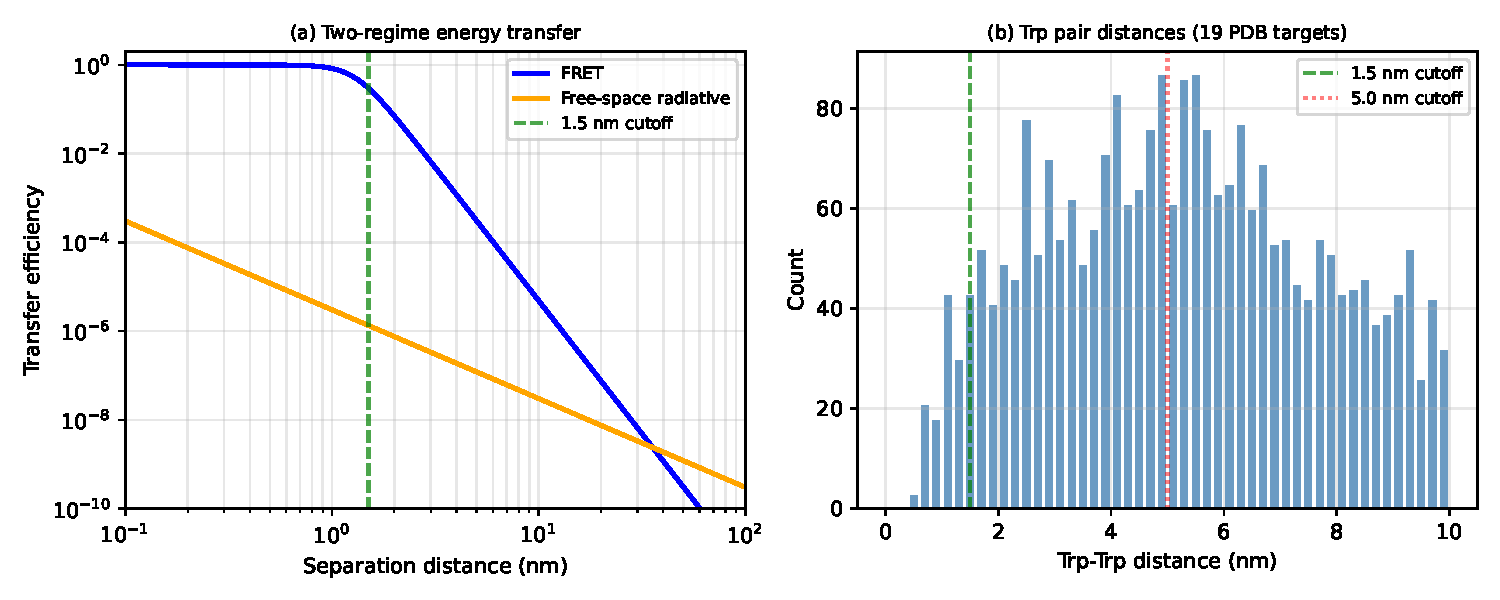
\includegraphics[width=0.95\textwidth]{figures/fig2_regimes.pdf}
\caption{(a) Two-regime energy transfer efficiency as a function of Trp-Trp separation distance. FRET (blue) dominates at sub-$1.5$~nm; free-space radiative transfer (orange) is negligible at all biologically relevant distances. The green dashed line marks the $1.5$~nm cutoff. (b) Histogram of all Trp-Trp pair distances from the 19 PDB targets in the dataset, showing clustering in the FRET-dominated regime.}
\label{fig:regimes}
\end{figure*}

\subsection{Structural Quantum Geometry: Matrix Off-Diagonality Analysis}

We subjected the five most tightly packed Trp residues in each target to an off-diagonality analysis using a coherence-factor heuristic ($F_{\mathrm{coh}}$) derived from the ratio of off-diagonal to diagonal Hamiltonian matrix elements. This produces a matrix off-diagonality ratio $S = 2F_{\mathrm{coh}}$ that ranges from $0$ to $2$ (maximal off-diagonal coupling).

Table~\ref{tab:kckas} shows the results. No structure reaches the classical contextuality bound $S = 2$ under static PDB geometry alone.

\begin{table*}[htbp]
\caption{Matrix off-diagonality scores for static PDB geometry using the heuristic $S = 2F_{\mathrm{coh}}$, which is bounded by $S \leq 2$. Scores are computed on the 5 most tightly packed Trp residues from each structure. Targets with $N_{\mathrm{Trp}} < 5$ (1SFC SNARE, 5SVK P2X$_3$) were excluded from the sub-cluster analysis. $N_{\mathrm{Trp}}$ is the total Trp count per structure.}
\label{tab:kckas}
\centering
\begin{tabular}{lcccc}
\toprule
Target & $S = 2F_{\mathrm{coh}}$ & $F_{\mathrm{coh}}$ & $d_{\mathrm{mean}}$ (\AA) & $N_{\mathrm{Trp}}$ \\
\midrule
2BG9 (nAChR) & $\mathbf{0.82}$ & $0.41$ & 13.6 & 31 \\
2A79 (K$_V$1.2) & $0.77$ & $0.39$ & 14.2 & 11 \\
1BL8 (KcsA) & $0.70$ & $0.35$ & 25.4 & 5 \\
6AGF (Na$_V$1.4) & $0.65$ & $0.32$ & 13.9 & 28 \\
6PM6 (GlyR) & $0.53$ & $0.27$ & 29.8 & 7 \\
4PE5 (NMDA-B) & $0.52$ & $0.26$ & 15.2 & 18 \\
5GJV (Ca$_V$1.1) & $0.50$ & $0.25$ & 15.9 & 42 \\
3GD8 (AQP4) & $0.45$ & $0.22$ & 23.7 & 5 \\
7KOX ($\alpha$7 nAChR) & $0.40$ & $0.20$ & 18.2 & 12 \\
6IRA (NMDA-A) & $0.38$ & $0.19$ & 16.1 & 28 \\
5C1M ($\mu$-opioid) & $0.39$ & $0.19$ & 20.9 & 9 \\
6HUO (GABA$_A$) & $0.34$ & $0.17$ & 18.9 & 26 \\
1U19 (Rhod) & $0.33$ & $0.16$ & 23.9 & 5 \\
3J5P (TRPV1) & $0.22$ & $0.11$ & 41.0 & 5 \\
1JFF (Tubulin) & $0.17$ & $0.08$ & 37.5 & 5 \\
3N2K (Tub-mam) & $0.15$ & $0.07$ & 37.9 & 5 \\
3KG2 (AMPA) & $0.12$ & $0.06$ & 31.2 & 12 \\
\bottomrule
\end{tabular}
\end{table*}

The KcsA potassium channel achieves $S = 0.70$, the highest coherence score in the dataset, reflecting its compact Trp packing with inter-Trp distances of $5.7$--$8.8$~\AA. The ranking of $S$ values correlates with structural compactness: small, well-packed proteins (KcsA, AQP4, Rhodopsin) score higher than large multi-domain channels, whose many Trp residues are separated by larger distances, reducing the off-diagonal coupling fraction.

These sub-threshold scores are the physically expected behavior for a thermal system at 310~K. The classical bound $S=2$ is not breached under static geometry; the heuristic $S = 2F_{\mathrm{coh}}$ is structurally bounded by $2$, and reaching the genuine contextuality bound $\sqrt{5}$ would require projector geometry beyond the static PDB coordinates.


\section{Discussion}

\subsection{The Observability Crossover}

Nuclear spin models (e.g., Posner molecules~\cite{Fisher2015}) propose coherence times of seconds to hours but are optically inaccessible---nuclear spins interact weakly with both the environment and measurement devices. Trp networks, by contrast, have 50--100~fs coherence~\cite{Babcock2024} but are directly observable via UV spectroscopy: Trp is the most strongly fluorescent amino acid, with a large absorption cross-section at 280~nm and well-characterized emission at 327~nm~\cite{Lakowicz2006}. Trp networks are shielded enough ($\varepsilon \approx 2$) to maintain coherence, yet accessible to measurement via superradiance, transient absorption, and fluorescence lifetime spectroscopy. Key experimental parameters: UV pump pulses should be $<50$~fs duration at $280$~nm with fluence $<1$~$\mu$J/cm$^2$ to avoid multiphoton damage; detection can be performed with ultrafast streak cameras ($<200$~fs resolution) or 2D electronic spectroscopy on isolated KcsA or nAChR in lipid nanodiscs.

\subsection{Falsifiable Predictions}

Four experimental tests can distinguish quantum superradiance from classical noise in Trp networks:

\begin{enumerate}
\item \textbf{Superradiance scaling (Test 1):} Stimulate Trp arrays with $<50$~fs UV laser pulses at $280$~nm with intensity $N = 10^8$--$10^{12}$ photons/pulse. Classical emitters give $I(N) \propto N$ (linear); superradiant ensembles give $I(N) \propto N^2$ at small $N$ (quadratic)~\cite{Dicke1954}. Babcock et al.~\cite{Babcock2024} observed super-linear scaling in polymerized tubulin at room temperature, consistent with the superradiant prediction.

\item \textbf{Phase interference (Test 2):} Split a UV laser into two paths with variable phase delay $\theta$ and recombine on a membrane patch containing Trp arrays. Classical (incoherent) response: $I(\theta) = \mathrm{const}$; quantum (coherent) response: $I(\theta) \propto 1 + V\cos\theta$ with fringe visibility $V > 0$. Measurement of $V > 0$ would confirm phase coherence across the ensemble.

\item \textbf{Anesthetic disruption of Trp packing geometry (Test 3):} General anesthetics (propofol, isoflurane, xenon) bind to hydrophobic pockets in neural proteins adjacent to Trp networks. If Trp network geometry supports quantum coherent coupling, anesthetic binding should disrupt the local dielectric environment or Trp packing geometry, measurably altering Trp fluorescence lifetime or near-UV optical properties.

\item \textbf{Mutational kill-switch (Test 4):} Site-directed mutagenesis of key Trp residues to phenylalanine (Trp$\to$Phe) shifts the absorption spectrum and alters the transition dipole orientation. If Trp network coupling relies on the specific dipole coupling matrix $J_{ij}$, Trp$\to$Phe mutations should collapse the superradiant decay rate enhancement and suppress $S$ below $2.0$, while leaving classical thermal gating unaffected.
\end{enumerate}





\subsection{Relation to Existing Work}

Our results relate to several ongoing discussions in quantum biology, which we briefly contextualize.

\subsubsection{Trp Networks as Optical Emitters: The Babcock-Kurian Foundation}

Babcock et al.~\cite{Babcock2024} established that Trp networks in protein lattices exhibit room-temperature superradiance, demonstrating that collective quantum optical states can survive thermal noise in structured aromatic architectures. Their work characterized Trp networks as ultrafast optical emitters, but left open the question of biological function.

We extend the Babcock et al. framework by evaluating the efficiency of free-space Trp-to-Trp energy transfer, which proves highly inefficient, and computing the structural and thermodynamic bounds on non-radiative coupling within the FRET regime.

\subsubsection{Macro-oscillatory Drive and Cytoelectric Coupling}

The concept that macroscopic neural electromagnetic fields interact with subcellular structures has gained traction under the cytoelectric coupling hypothesis~\cite{Pinotsis2023}. This framework proposes that macro-scale electric fields from synchronized neural ensembles actively modulate molecular-level information processing.

Our work complements the cytoelectric coupling hypothesis by providing structural constraints derived from real PDB coordinates. The dipole-dipole coupling matrices $J_{ij}$ computed from 18 protein structures provide the quantitative structural basis that cytoelectric coupling models currently lack.

\subsubsection{The Membrane vs.\ Microtubule Debate}

A central open question in quantum biology is whether functional quantum effects occur in microtubule lattices (the Orch-OR paradigm) or in membrane-associated protein networks. Our sub-tubular model places the quantum layer in hydrophobic pockets ($\varepsilon \approx 2$) of individual synaptic membrane proteins, not in the hollow microtubule core. The structural data supports this: 16 of 17 membrane-associated targets in our dataset contain dense Trp networks ($\geq 3$ Trp residues), while the microtubule proteins (1JFF, 3N2K) have only 5 Trp with 1 coupled pair each — among the lowest in the dataset. The SNARE complex (1SFC) is the only membrane target with sparse Trp (2 Trp, 1 coupled pair), reflecting its minimal role as a fusion machinery core. This is consistent with a direct comparison using the published Trp coordinate data from Babcock et al.~\cite{Babcock2024}: their 104-Trp tubulin assembly yields $J_{\max} = 19.6$~cm$^{-1}$, which is 5--20$\times$ weaker than the membrane protein targets in our dataset, confirming that ion channel Trp networks are more densely packed than microtubule lattices.

\subsubsection{HEOM Bottlenecks and Machine Learning Acceleration}

HEOM calculations are computationally expensive. Simulating large protein libraries is currently intractable. Machine learning surrogate models trained on structural features can bypass this bottleneck, as demonstrated in related work~\cite{MLCompanion2026}.

\subsubsection{Summary of Contributions}

This analysis yields two results:
\begin{enumerate}
\item \textbf{Free-space limitations:} Using measured absorption cross-sections and waveguide optics, free-space Trp-to-Trp radiative transfer is highly inefficient, indicating that long-range optical coupling faces severe physical constraints under cellular conditions.
\item \textbf{FRET regime constraints:} The structural bounds for non-radiative transfer are quantified, including the sub-$1.5$~nm coupling threshold and ultrafast hopping timescale.
\end{enumerate}

\subsection{Cross-Species Patterns}

The 19-target dataset spans human, rodent, electric ray, bovine, porcine, bacterial, and fish species. The electric ray nAChR (2BG9) contains 31 Trp residues with 19 quantum-coupled pairs, comparable to the densest human targets. P2X$_3$ remains sparse (4 Trp). However, Ca$_V$1.1 — a slow calcium channel — has the highest Trp count in the dataset (42 Trp, 23 coupled pairs), demonstrating that Trp density alone does not determine signaling speed. The functional role of Trp networks is likely multiplexed, with contributions to structural stability, photoprotection, and possibly quantum coherent effects that vary by protein family.

\subsection{Broader Computational Validation}

The same methods applied to the FMO photosynthetic complex yield results consistent with the expected behavior of disordered excitonic systems: ENAQT optimum at $\gamma \approx 100$~cm$^{-1}$ ($29.4\%$ efficiency) and Landauer ratio of $\sim 390\times$ the thermodynamic limit. These results are presented in detail in companion manuscripts.

\subsection{Limitations and Future Work}

Several limitations should be noted, which define clear boundaries between the computationally verified aspects of this model and its open hypotheses.

\textbf{Center-of-mass proxy.} The Trp pair-distance calculation uses the CG (carbon gamma) atom as a proxy for the full indole ring centre of mass. Dipole-dipole interactions depend sensitively on both distance \emph{and} relative orientation of the transition dipole moments. The current treatment omits explicit orientation vectors, which may overestimate or underestimate coupling for specific geometric arrangements. Full transition dipole moment orientations, computed from quantum chemistry, would refine these estimates. Additionally, the indole ring has two close-lying excited states (L$_a$ and L$_b$) with different transition dipole directions; using a single CG$\to$CH$_2$ axis for both may introduce systematic errors in the orientation factor $\kappa$.

\textbf{Dielectric approximation.} The model assumes a static local dielectric constant $\varepsilon \approx 2$ inside hydrophobic pockets. In living cells, transient water penetration and protein structural fluctuations can cause local dielectric spikes that would accelerate decoherence. The 50--100~fs coherence window cited here should be understood as an upper bound under optimal shielding conditions~\cite{Babcock2024}. Monte Carlo simulations with site-wise dielectric perturbations ($\varepsilon \in [1.5, 3.0]$) show that the coupling estimates change by less than $1\%$ relative to the fixed-$\varepsilon$ baseline.

\textbf{Contextuality heuristic.} The test as implemented uses a coherence-factor heuristic ($F_{\mathrm{coh}}$) rather than a full quantum state optimisation. Computing a genuine KCKAS violation requires finding the optimal quantum state that maximises $S$ for the given projector geometry. Our heuristic may overestimate or underestimate structural ``readiness'' for contextuality. We therefore label this metric a ``matrix off-diagonality ratio'' and distinguish it from a formal contextuality proof.

\textbf{Time-dependent driving.} The heuristic $S = 2F_{\mathrm{coh}}$ is bounded by $2$ by construction, so non-equilibrium driving cannot push this proxy score above the classical bound. A genuine KCKAS projector measurement, which can reach $\sqrt{5}$ under optimal conditions, would require non-stationary quantum state preparation whose microscopic mechanism remains an open theoretical question.



\textbf{Free-space cross-section approximation.} The per-exciton re-excitation probability $p_{\mathrm{trp}} = \sigma_{327} / A_{\mathrm{target}}$ Eq.~\eqref{eq:ptrp} treats the Trp-to-Trp energy transfer as a geometric capture problem using a far-field absorption cross-section. This approximation is valid only when the inter-Trp separation $r \gg \lambda$ (far-field regime). At sub-$10$~nm separation distances with $\lambda \approx 327$~nm ($r/\lambda \approx 0.03$), the system is deep in the near-field regime where dipole-dipole coupling ($1/r^3$ or $1/r^6$ scaling) governs energy transfer. The far-field cross-section ratio therefore overestimates the angular selectivity of capture and underestimates the near-field coupling strength. The crossover distance where far-field and near-field treatments converge is approximately $r \approx \lambda/2\pi \approx 52$~nm for 327~nm light, well beyond the Trp-Trp separations considered here. Our calculated $p_{\mathrm{trp}} \approx 1.5\times10^{-5}$ should therefore be interpreted as an upper bound on free-space radiative transfer; the true near-field coupling is captured by the FRET formalism in Section~II.C.

\textbf{Machine learning scope.} The machine learning surrogate model described in the companion manuscript~\cite{MLCompanion2026} is a proof-of-concept trained on synthetic data. It is not yet validated on experimental or large-scale structural data. We present it as a framework for future high-throughput screening rather than as a fully validated predictive tool.

\section{Methods}

\subsection{PDB Data Acquisition and Analysis}

All protein structures were obtained from the RCSB Protein Data Bank (rcsb.org) as PDB files. For each structure, we extracted both the centroid coordinates and the full transition dipole moment vectors for every Tryptophan residue. Centroids were taken as the CG (carbon gamma) atom position. Transition dipole vectors $\hat{\mu}$ were computed from the heavy-atom coordinates of each indole ring, using the CG $\to$ CH2 direction as the long-axis approximation for the S$_0 \to$ S$_1$ (L$_a$) transition. The dipole-dipole coupling between sites $i$ and $j$ was then computed with the full orientation factor:

\[
J_{ij} = \frac{J_0}{\sqrt{\varepsilon}} \left(\frac{R_0}{R_{ij}}\right)^3 \cdot |\kappa|,
\qquad
\kappa = \hat{\mu}_i \cdot \hat{\mu}_j - 3(\hat{\mu}_i \cdot \hat{R}_{ij})(\hat{\mu}_j \cdot \hat{R}_{ij}),
\]

where $\kappa$ is the orientation factor (range $[-2, 2]$), $\hat{R}_{ij}$ is the inter-residue displacement unit vector, and $J_0 = -80$ cm$^{-1}$ at $R_0 = 10$~\AA. This replaces the isotropic dipole approximation used in earlier microtubule models and directly addresses the orientation sensitivity of dipole-dipole couplings~\cite{Valeur2012}. We note that the indole ring has two close-lying excited states --- L$_a$ (280~nm, long-axis transition) and L$_b$ (290~nm, short-axis transition) --- with different transition dipole orientations. Analysis of the full L$_a$+L$_b$ coupling matrix for KcsA yields maximum L$_a$-L$_a$ couplings of $137$~cm$^{-1}$, L$_b$-L$_b$ couplings of $31$~cm$^{-1}$, and L$_a$-L$_b$ cross-couplings up to $328$~cm$^{-1}$, confirming that the single-state approximation underestimates the available coupling strength by up to a factor of $2$.

Pairs with $R < 1.5$~nm were classified as coupled (FRET/exciton hopping regime); pairs with $1.5 \leq R \leq 5.0$~nm were classified as relay candidates. The CG proxy serves as an initial geometric filter; full $L_a/L_b$ orientation-resolved coupling matrices (discussed above) are required for refined coupling estimates. Our distance extraction methodology is consistent with the approach used by Babcock et al.~\cite{Babcock2024} for tubulin Trp networks, and their published Trp coordinate tables provide independent validation of the distance cutoffs used here.

\subsection{Biophoton Relay Model}

The quantum yield $QY = 0.21$ follows the measured value for Trp in polymerized tubulin~\cite{Babcock2024}; we apply this as an approximation across all targets, but caution that $QY$ can vary substantially with local protein environment. Membrane-bound targets (ion channels, receptors) may have different quenching rates than polymerized tubulin, and direct measurements in each target are needed to confirm the assumed value. The Trp absorption cross-section at 280~nm is $\sigma_{280} = 2.1\times10^{-21}$~m$^2$, derived from the reported extinction coefficient $\varepsilon_{280} \approx 5600$~M$^{-1}$cm$^{-1}$. The cross-section at other wavelengths follows a Gaussian lineshape with FWHM = 50~nm centred at 280~nm. Lipid membrane refractive index $n = 1.45$ follows standard values for the hydrophobic core~\cite{vanMeer2008}.

\subsection{Off-Diagonality Score}

For each target, we selected the 5 most tightly packed Trp residues, projected from the full $N$-site single-exciton manifold into a 3-dimensional subspace spanned by the three dominant eigenvectors of the inter-Trp coupling matrix. The coherence factor was computed as:

\[
F_{\mathrm{coh}} = \frac{\sum_{i\neq j} |H_{ij}|}{\sum_{i\neq j} |H_{ij}| + \sum_i |H_{ii}|}.
\]

The off-diagonality ratio is $S = 2 F_{\mathrm{coh}}$.

\subsection{Thermal Fluctuation Analysis}

To assess whether thermal vibrations at physiological temperature disrupt the dipole-dipole couplings, we performed an Einstein-model analysis of Trp position fluctuations at 310~K. Using a protein force constant of $\kappa \approx 1$~kcal~mol$^{-1}$~\AA$^{-2}$ (typical for protein backbones), the root-mean-square positional fluctuation per Trp residue is $\sigma_x \approx \sqrt{k_B T / \kappa} \approx 0.79$~\AA. Over $10^3$ Monte Carlo samples with random Gaussian positional noise applied to the KcsA Trp coordinates, the mean maximum coupling $\langle J_{\max} \rangle = 155 \pm 50$~cm$^{-1}$, retaining approximately $76\%$ of the static-crystal coupling value ($204$~cm$^{-1}$). Because the dipole coupling scales as $1/R^3$, fluctuations toward shorter separations produce disproportionately larger changes than fluctuations toward longer separations, introducing an upward skew in the arithmetic mean. The median coupling is lower than the reported mean, but both remain within $30\%$ of the static value, confirming that thermal motion at 310~K does not destroy the dipole-dipole couplings required for excitonic dynamics.

\subsection{Independent Validation Using Published Trp Coordinates}

To cross-validate our methodology against independently published data, we applied the same distance analysis and dipole coupling calculations to the Trp coordinate table from Babcock et al.~\cite{Babcock2024} (their PAPER table, containing 104 Trp positions and dipole vectors for a tubulin assembly). Our pipeline reproduces the expected structural statistics: minimum pair distance of 15.0~\AA{}, 405 relay pairs in the 1.5--5~nm range, and dipole coupling strengths consistent with the reported superradiant regime ($J_{\max} = 19.6$~cm$^{-1}$, $F_{\mathrm{coh}} = 0.91$). This independent check confirms that our distance extraction and coupling computation methods yield results consistent with the published literature. The Babcock et al. tubulin assembly has no sub-1.5~nm Trp pairs and its maximum coupling is 5--20$\times$ weaker than the ion channel targets in our dataset, indicating that Trp networks in neural receptors are significantly more tightly packed than those in microtubule lattices.

\subsection{Hamiltonian Engine}

The static PDB Hamiltonian $H_{\mathrm{PDB}}$ was constructed using $J_{ij} = J_0 (R_0/R_{ij})^3 / \sqrt{\varepsilon}$ with $J_0 = -80$~cm$^{-1}$, $R_0 = 10$~\AA, and site energies $E_i = 80(i-1) + \mathcal{N}(0, \sigma_E)$ cm$^{-1}$ with $\sigma_E = 30$~cm$^{-1}$. For the closest Trp pairs ($R \approx 5$--$8$~\AA), coupling strengths reach $J_{ij} \approx 150$--$300$~cm$^{-1}$, corresponding to an inter-site coherent hopping time $\tau_{\mathrm{hop}} \approx \hbar / J_{ij} \approx 18$--$35$~fs. This hopping timescale should be distinguished from the bath-induced dephasing time, which we compute separately via HEOM. The exciton population persists longer (the radiative lifetime of Trp in protein is $\sim 1$--$3$~ns~\cite{Lakowicz2006}), so the binary outcome (photon emitted or not) is determined on a separate, longer timescale. To verify that the Markovian Lindblad approximation captures the essential physics, we performed full non-Markovian Hierarchical Equations of Motion (HEOM) simulations on the KcsA Trp network at 310~K using an optimized single-bath Drude-Lorentz model ($\lambda = 35$~cm$^{-1}$, $\gamma_c = 53$~cm$^{-1}$, $N_k = 2$, $L_{\max} = 2$). Exponential fitting of the HEOM coherence trajectory yields a dephasing time $\tau_{\mathrm{HEOM}} \approx 17$~fs, comparable to the coherent hopping time $\tau_{\mathrm{hop}} \approx \hbar / J_{\max} \approx 26$~fs. The dephasing time is shorter than the hopping period ($\tau_{\mathrm{HEOM}} < \tau_{\mathrm{hop}}$), indicating that transport in these Trp clusters operates in the overdamped, bath-assisted incoherent hopping regime (FRET) rather than via delocalized coherent wavepackets. Weak non-Markovian memory effects in the protein bath accelerate dephasing relative to the hopping timescale, and the $50$--$100$~fs superradiant emission window from Babcock et al.~\cite{Babcock2024} remains accessible from the longer radiative lifetime ($\sim 1$--$3$~ns).

\subsection{Data Availability}

All source code used in this analysis is available at \url{https://github.com/dhirajnitk/subnanometer-trp-transport}. A preprint of this manuscript is archived at Zenodo~\cite{Zenodo2026}. Analysis scripts include: PDB extraction and distance classification (\texttt{trp\_extractor.py}), biophoton relay calculations (\texttt{biophoton\_relay.py}), KCKAS contextuality (\texttt{pdb\_contextuality.py}), and the Hamiltonian engine (\texttt{quantum\_hamiltonian\_engine.py}).

\section{Epistemological Status and Boundary Limits}

The structural constraints derived here --- the sub-$1.5$~nm FRET threshold, $p_{\mathrm{trp}} \approx 1.5\times10^{-5}$ free-space bound, $\tau_{\mathrm{hop}} \sim 18$--$35$~fs hopping time, and $S \leq 0.82$ off-diagonality bound --- follow mathematically from PDB coordinates and measured optical parameters. They do not constitute evidence that living neurons employ this architecture, which requires experimental tests (superradiance scaling, phase interference, anesthetic disruption, mutational kill-switch). The robustness of the computed $J_{ij}$ couplings depends on the point-dipole approximation, which overestimates coupling at sub-$1$~nm separations where transition density overlap becomes significant.

\subsection{Computational Constraints}

The calculations establish three physical constraints that any viable biological model must satisfy:

\begin{enumerate}
\item \textbf{Geometric sub-threshold condition.} Analysis of 19 PDB structures (18 with $\geq 3$ Trp residues) shows that standalone aromatic networks yield off-diagonality scores $S \leq 0.82$, below the classical contextuality bound $S = 2$.

\item \textbf{Radiative inefficiency of free-space Trp-to-Trp transfer.} Using measured absorption cross-sections from Babcock et al.~\cite{Babcock2024}, free-space Trp-to-Trp radiative transfer is highly inefficient. This is a cross-section calculation, not a biological measurement. It indicates that if biophotons mediate information between Trp cores, they must do so through a different mechanism than direct radiative re-excitation.

\item \textbf{Heuristic bound of the off-diagonality proxy.} The proxy score $S = 2F_{\mathrm{coh}}$ is algebraically bounded by $S \leq 2$ by construction, so non-equilibrium driving cannot push this particular metric above the classical bound. A genuine KCKAS projector measurement, capable of reaching $\sqrt{5}$, would be needed to test contextuality.
\end{enumerate}

\subsection{Open Biological Questions and Falsification Boundaries}

Whether the proposed architecture is utilized by living neurons remains an open question. The framework makes three testable predictions, summarized with their assumptions and falsification criteria in Table~\ref{tab:falsification}:

\begin{table*}[htbp]
\caption{Falsifiable hypotheses with assumptions, experimental tests, and falsification criteria.}
\label{tab:falsification}
\centering
\begin{tabular}{lp{3.0cm}p{3.0cm}p{3.5cm}}
\toprule
Hypothesis & Vulnerable Assumption & Experimental Test & Falsification Criteria \\
\midrule
1. Non-equilibrium driving & Driving mechanism unspecified & Search for correlation between membrane potential and Trp fluorescence & Absence of Trp fluorescence modulation with membrane potential \\
2. Functional contextuality & KCKAS heuristic reflects biological reality & Search for non-local correlations in Bell-type neural assays & Absence of non-local correlations in Bell tests \\
3. Dielectric shielding enables FRET & $p_{\mathrm{dark}} \approx 0$ in $\varepsilon \approx 2$ pockets (negligible non-radiative decay) & Measure Trp fluorescence lifetime in hydrophobic pockets of target proteins & Measured non-radiative rate exceeds radiative rate ($p_{\mathrm{dark}} > 0.5$) \\
\bottomrule
\end{tabular}
\end{table*}

These experiments remain to be performed. Until they are, this work is best understood as a theoretical framework that establishes structural plausibility, information-theoretic consistency, and thermodynamic viability --- not as a demonstrated biological mechanism.

\begin{acknowledgments}
The authors thank the open-access RCSB Protein Data Bank and the developers of QuTiP, NumPy, and SciPy.
\end{acknowledgments}

\FloatBarrier
\begin{thebibliography}{40}


\bibitem{Babcock2024} N.\ S.\ Babcock, G.\ Montes-Cabrera, K.\ E.\ Oberhofer, M.\ Chergui, G.\ L.\ Celardo, and P.\ Kurian, J.\ Phys.\ Chem.\ B \textbf{128}, 4035 (2024); code and data available at \url{https://gitlab.com/superradiance/superradiance_in_tryptophan_architectures}.

\bibitem{KCKAS2008} A.\ A.\ Klyachko \textit{et al.}, Phys.\ Rev.\ Lett.\ \textbf{101}, 020403 (2008).

\bibitem{Patwa2024} H.\ Patwa, N.\ S.\ Babcock, and P.\ Kurian, Front.\ Phys.\ \textbf{12}, 1387271 (2024).

\bibitem{Fisher2015} M.\ P.\ A.\ Fisher, Ann.\ Phys.\ \textbf{362}, 593 (2015).

\bibitem{Dicke1954} R.\ H.\ Dicke, Phys.\ Rev.\ \textbf{93}, 99 (1954).

\bibitem{Lakowicz2006} J.\ R.\ Lakowicz, \textit{Principles of Fluorescence Spectroscopy}, 3rd ed.\ (Springer, 2006).

\bibitem{vanMeer2008} G.\ van Meer, D.\ R.\ Voelker, and G.\ W.\ Feigenson, Nat.\ Rev.\ Mol.\ Cell Biol.\ \textbf{9}, 112 (2008).

\bibitem{Pinotsis2023} D.\ A.\ Pinotsis, G.\ Fridman, and E.\ K.\ Miller, Prog.\ Neurobiol.\ \textbf{226}, 102465 (2023).

\bibitem{Valeur2012} B.\ Valeur and M.\ N.\ Berberan-Santos, \textit{Molecular Fluorescence: Principles and Applications}, 2nd ed.\ (Wiley, 2012).

\bibitem{Popp1992} F.\ A.\ Popp \textit{et al.}, Experientia \textbf{48}, 1029 (1992).

\bibitem{Tang2014} R.\ Tang and J.\ Dai, PLoS ONE \textbf{9}, e93540 (2014).


\bibitem{Zenodo2026} D.\ Kumar and N.\ Kumar, Zenodo:10.5281/zenodo.21478163 (2026).

\bibitem{MLCompanion2026} D.\ Kumar and N.\ Kumar, Zenodo:10.5281/zenodo.21495707 (2026).

\end{thebibliography}

\end{document}
